\makeatletter
\def\input@path{{ieee_access_official_templates/latex/ACCESS_latex_template_20260513/}{./}}
\makeatother
\documentclass{ieeeaccess}
% Official IEEE Access class (ieeeaccess.cls from ieeeaccess.ieee.org, 2026-05-13 LaTeX bundle).
% Scientific content is transcribed from docs/paper/IEEE_TEMPLATE_READY_MANUSCRIPT.md.
% Do not treat this file as a source of new experimental results.
\usepackage{cite}
\usepackage{amsmath,amssymb,amsfonts}
\usepackage{graphicx}
\usepackage{textcomp}
\usepackage{array}
\usepackage{tabularx}
\usepackage{booktabs}
\usepackage{microtype}
% Layout-only helpers: wrap SHA-256 and long identifiers inside a column
% without truncating or altering characters. Robust for tabularx trials.
\makeatletter
\DeclareRobustCommand{\sha}[1]{{\ttfamily\expandafter\@shaloop\detokenize{#1}\relax}}
\def\@shaloop#1{%
  \ifx\relax#1\else#1\allowbreak\expandafter\@shaloop\fi}
\makeatother
\renewcommand{\arraystretch}{1.18}
\setlength{\tabcolsep}{3.5pt}
\usepackage{bm}
\makeatletter
\AtBeginDocument{\DeclareMathVersion{bold}
\SetSymbolFont{operators}{bold}{T1}{times}{b}{n}
\SetSymbolFont{NewLetters}{bold}{T1}{times}{b}{it}
\SetMathAlphabet{\mathrm}{bold}{T1}{times}{b}{n}
\SetMathAlphabet{\mathit}{bold}{T1}{times}{b}{it}
\SetMathAlphabet{\mathbf}{bold}{T1}{times}{b}{n}
\SetMathAlphabet{\mathtt}{bold}{OT1}{pcr}{b}{n}
\SetSymbolFont{symbols}{bold}{OMS}{cmsy}{b}{n}
\renewcommand\boldmath{\@nomath\boldmath\mathversion{bold}}}
\makeatother
\graphicspath{{figures/}{../../../figures/}{ieee_access_official_templates/latex/ACCESS_latex_template_20260513/}{./}}

\def\BibTeX{{\rm B\kern-.05em{\sc i\kern-.025em b}\kern-.08em
    T\kern-.1667em\lower.7ex\hbox{E}\kern-.125emX}}

\begin{document}
% Author-review / pre-acceptance PDF: no invented publication date, DOI, or volume/year.
% Do not invent a DOI. IEEE Access assigns official metadata upon acceptance/publication.
\title{Evidence-Separated Credit Scoring, Additive Explainability, and Shariah-Oriented Governance: A Research Prototype on a LendingClub Extract, with Independent UCI Methodology Context}
\author{\uppercase{Aitsam Ul Hassan}\authorrefmark{1} and \uppercase{Muhammad Haseeb Ramzan}\authorrefmark{1}}
\address[1]{Pak-Austria Fachhochschule: Institute of Applied Sciences and Technology, Haripur, Pakistan (e-mails: aitsamulhassan.awan@gmail.com; haseebramzan536@gmail.com)}
\corresp{Corresponding author: Aitsam Ul Hassan (e-mail: aitsamulhassan.awan@gmail.com).}
% Funding/sponsor footnote omitted: not supplied; not invented.
% ORCID omitted: not supplied for either author; not invented.

\markboth{}{}
\makeatletter
% Suppress sample history/DOI line and template VOLUME/logo headers for this author-review PDF.
\long\def\@maketitle{%
  \setbox\maketitlebox\hbox\bgroup
  \begin{minipage}{\titlewidth}%
  \raggedright\vspace*{1.2mm}%
  {\vss\color{accessblue}\titlefont\@title\vss}\vspace*{6mm}\par
  \ifaccesseditors\vspace*{2mm}\else{\vss\authorfont\@author\vss}\vspace*{0mm}\par
  \@tempcnta=0%
  \loop\ifnum\@tempcnta<\theaddrCtr
    \advance\@tempcnta by 1%
    \par{\vss\addressfont\textsuperscript{\expandafter\csname addrInd\the\@tempcnta\endcsname}%
     \expandafter\csname addr\the\@tempcnta\endcsname\vss}%
  \repeat\vspace*{1mm}\par
  {\vss\correspfont\@corresp\vss\vspace{2mm}}\par\fi
  {\vss\tfootnotefont\@tfootnote\vss\vspace{7mm}}\par
  \noindent\box99\vspace{6mm}\par
  \ifaccesseditors\vspace*{8mm}\else
  \noindent\box88\vspace{18mm}\par
  \fi
  \end{minipage}\par
  \egroup
  \box\maketitlebox
  \vspace*{3.5pt}%
  \vspace*{\titlepgskip}%
}
\def\ps@headings{%
  \def\@oddhead{\hfill}%
  \def\@evenhead{\hfill}%
  \def\@oddfoot{%
    \hbox to \textwidth{\hfill{\footerpagefont\thepage}\hfill}}%
  \def\@evenfoot{%
    \hbox to \textwidth{\hfill{\footerpagefont\thepage}\hfill}}%
}
\def\ps@titlepage{%
  \def\@oddhead{\hfill}%
  \def\@evenhead{\hfill}%
  \def\@oddfoot{%
    \hbox to \textwidth{\hfill{\footerpagefont\thepage}\hfill}}%
  \def\@evenfoot{%
    \hbox to \textwidth{\hfill{\footerpagefont\thepage}\hfill}}%
}
\ps@headings
\makeatother


\begin{abstract}
This study presents a research prototype that separates credit-risk scoring, additive explainability, and Shariah-oriented governance evidence, and fuses them only at a frozen decision map. It is not Shariah certification, a fatwa, an automated compliance verdict, expert-validated Shariah decisioning, or a production credit engine, and it reports no fraud-detection performance. The primary dataset is a Zenodo LendingClub granting-model extract of 1,347,681 originated-and-resolved loans (US peer-to-peer, 2007--2018; not an Islamic-finance sample), with 941,267 training, 197,528 validation, and 208,886 test loans. Four LendingClub families---logistic regression, random forest, XGBoost, and an additive explainable boosting machine (EBM) with no interactions---were test-evaluated after a training-plus-validation refit (context M-4B); validation selected the EBM. Downstream probabilities come from a distinct training-only EBM with validation-only Platt scaling (context M-5). On the frozen test set, M-5 raw and Platt receiver-operating-characteristic area under the curve (ROC-AUC) both equal 0.6776693941139847; Platt Brier score is 0.15616920271522994 and expected calibration error (ECE) is 0.020267295489117824. The test set was not used to fit calibration. Explanations use an exact additive SHAP-style logit decomposition of the M-5 EBM; TreeSHAP was not used. The extract lacks contract-level Shariah fields. Dataset-level status is INSUFFICIENT\_SCHEMA\_FOR\_APPLICANT\_DETERMINATION; all 208,886 test rows receive INSUFFICIENT\_INFORMATION---an evidence-schema limitation, not a compliance verdict. Frozen-score research maps assign 5,232 / 203,627 / 27, 0 / 208,859 / 27, and 61,855 / 0 / 147,031 approve / human-review / reject decisions under credit-only, fused, and single-threshold rules; predictive scores are identical across maps. Independent UCI logistic-regression and EBM results are methodology context only; UCI XGBoost is exploratory.
\end{abstract}

\begin{keywords}
credit risk, evidence traceability, explainable boosting machine, probability calibration, Shariah-oriented governance.
\end{keywords}

\titlepgskip=-21pt
\maketitle

\section{Introduction}
\label{sec:introduction}

\PARstart{C}{onsumer} credit scoring is a statistical classification of applicants into higher- versus lower-risk classes \cite{b1}. Machine-learning classifiers have been benchmarked against traditional scorecards on institutional credit data \cite{b2}, \cite{b3}. Separately, probability-of-default estimation has been argued to be more decision-relevant than a binary good/bad label in credit-card default research \cite{b4}. Peer-to-peer (P2P) lending extracts from the Lending Club platform have been used in prior risk and explainability studies \cite{b5}, \cite{b6}; those studies do not evaluate the Zenodo granting-model extract executed here \cite{b20}.

Two further literatures motivate the design of this prototype, without validating its test-set metrics. First, post-hoc probability calibration (sigmoid / Platt scaling and isotonic regression) is a standard method for mapping classifier scores to probabilities \cite{b14,b15,b16}, and expected calibration error is a documented reliability summary \cite{b17}. Second, generalized additive models (GAMs) and glass-box boosting implementations provide additive structure that can be inspected feature-wise \cite{b9,b10,b11}. Additive SHAP attributions are defined for that class of explanations \cite{b12}; TreeSHAP is designed for tree ensembles rather than a first-order GAM \cite{b13}.

A third motivation is governance and auditability rather than predictive gain. US adverse-action rules require specific principal reasons, including when complex algorithms are used \cite{b32,b33,b34}. Those instruments apply to US creditors; this study is a research prototype and is not presented as an Equal Credit Opportunity Act (ECOA) originator or as a compliance guarantee. In Islamic finance, official Shariah governance frameworks for Islamic banking institutions in Pakistan and related documentary-evidence circulars describe board-level product approval and contract-level evidence requirements \cite{b24,b25,b26}. Separately, IFSB-10 records guiding principles for Shariah governance systems of institutions offering Islamic financial services \cite{b31}; it is cited as identity/FAQ context, not as a Pakistan Islamic-banking-institution circular and not as a ruling on this extract. Securities regulation in Pakistan further states that a security shall not be called Shariah compliant unless a Commission certificate is granted \cite{b27}. Those instruments do not license this software to certify loans in the executed LendingClub extract.

The executed design question is:

\begin{quote}
Does separating credit-risk scoring, explainability, and Shariah-oriented governance into independently validated and auditable evidence layers, fused only at the final decision stage, provide a more transparent and defensible digital-financing pipeline than a monolithic end-to-end classifier without materially sacrificing predictive performance?
\end{quote}

This paper treats that sentence as a \textbf{design question}, not as a proven operational-superiority result. On frozen calibrated probabilities, decision counts differ across maps while predictive scores remain identical. Governance is not claimed to improve ROC-AUC.

The evaluation examines two executed datasets only: the Zenodo LendingClub granting-model extract as the primary setting \cite{b20}, and the UCI Default of Credit Card Clients table as an independent credit/calibration methodology context \cite{b4}, \cite{b21}. German Credit and Australian Credit Approval are common literature benchmarks \cite{b22}, \cite{b23} and were \textbf{not} executed. No fraud-detection experiment was executed; fraud detection is a distinct statistical task \cite{b19} and is not reported as a performance result of this study.

The remainder of this paper is organized as follows. Section II reviews related work. Section III states research-gap and contribution boundaries. Section IV describes methods. Section V records the experimental protocol and authorization classes. Section VI transcribes stored results. Sections VII--IX discuss, limit, and conclude.


\section{Related Work}

Literature is used for methodological motivation and comparison with prior research. It is \textbf{not} used to claim that this project's test-set metrics have been independently validated. No 2023--2026 systematic review of machine-learning credit scoring was locked in the recorded literature sources; related work therefore uses the verified 1997--2022 scholarly sources and the recorded regulatory/standard instruments. No verified paper on real-time latency or throughput of loan engines was recorded; automated-lending discussion uses regulatory texts rather than systems-performance literature.

\subsection{Credit Scoring and Machine-Learning Benchmarks}

Hand and Henley review statistical classification methods for consumer credit scoring and note that commercial scorecard detail is often unpublished \cite{b1}. Baesens \emph{et al.} benchmark classification algorithms on real credit datasets \cite{b2}. Lessmann \emph{et al.} update that benchmark with later algorithms and performance measures \cite{b3}. Those populations, periods, and pipelines differ from the executed LendingClub extract. They do not rank the models in this study.

Yeh and Lien compare data-mining techniques for probability of default on Taiwan credit-card clients and argue for reporting estimated default probabilities \cite{b4}. The corresponding UCI record is dataset 350 \cite{b21}. That table is the independent secondary dataset in this project. Yeh and Lien's ranking of methods on their metric is \textbf{their} result, not this project's UCI analysis.

Malekipirbazari and Aksakalli study random-forest risk assessment on Lending Club platform data \cite{b5}. Ariza-Garzón \emph{et al.} study SHAP explanations of a P2P granting scoring model \cite{b6}. Those papers provide literature context for Lending Club / P2P modeling. They do not use the hashed Zenodo granting-model extract executed here \cite{b20}, and they do not confirm this project's additive EBM attributions.

Common public credit benchmarks also include German Credit (UCI Statlog, \(n=1000\)) \cite{b22} and Australian Credit Approval (UCI Statlog, \(n=690\)) \cite{b23}. They appear here only as literature-context datasets. They were not acquired as executed study files and must not be read as additional empirical settings of this prototype.

\subsection{Explainable Models and Additive Attributions}

Hastie and Tibshirani formulate GAMs as additive smooth functions of individual features \cite{b9}. Lou \emph{et al.} describe GA2M models that may add pairwise interactions while remaining visualizable \cite{b10}. Nori \emph{et al.} describe the Explainable Boosting Machine in InterpretML as a glass-box cyclic gradient-boosted GAM \cite{b11}. The present study froze EBM \texttt{interactions=0}; pairwise GA2M terms were not fitted to improve test-set scores. Citation of \cite{b10} is family background, not evidence that interactions were used.

Lundberg and Lee define SHAP additive feature attributions \cite{b12}. Lundberg \emph{et al.} present TreeSHAP / TreeExplainer for trees, forests, and gradient-boosted trees \cite{b13}. TreeSHAP is not an appropriate explainer for a first-order EBM GAM; this project did not use it. Bussmann \emph{et al.} apply Shapley-style explanations in an SME P2P credit-risk setting \cite{b7}. That population differs from the executed Zenodo LendingClub granting-model extract, and their pipeline is not this project's closed-form centered-term identity.

\subsection{Probability Calibration}

Platt describes a sigmoid map from classifier scores to probabilities \cite{b14}. The recorded literature sources include \textbf{no DOI} for that chapter and do not verify an official publisher URL; identity is retained as recorded. Niculescu-Mizil and Caruana compare Platt scaling and isotonic regression \cite{b15}. Zadrozny and Elkan describe isotonic-style calibration of ranking scores \cite{b16}. Guo \emph{et al.} discuss calibration and ECE for modern neural networks on vision and document tasks \cite{b17}; that population is not credit scoring. These papers motivate calibration candidates. They do not supply the frozen Platt parameters \(a\) and \(b\), and they do not validate the stored test-set Brier score or ECE.

\subsection{Boosting Algorithms}

Chen and Guestrin describe XGBoost as a scalable tree-boosting system \cite{b18}. That citation is an algorithm description. It does not merge LendingClub XGBoost (context M-4B) with UCI XGBoost (context M-9.4-X), and it does not make the exploratory UCI XGBoost analysis confirmatory or overall superior.

\subsection{Fraud Detection (Literature Context Only)}

Bolton and Hand review statistical fraud detection as a task distinct from ordinary default prediction \cite{b19}. This project executed no fraud experiment. Literature \cite{b19} supports a \textbf{negative} claim: fraud-detection performance is not reported.

\subsection{Fairness, Auditability, and Automated Lending}

Kozodoi, Jacob, and Lessmann study fairness criteria in credit scoring and document profit trade-offs \cite{b8}. This project did not execute fairness processors. Citation of \cite{b8} is related-work context only.

US Regulation B requires written adverse-action notices with specific principal reasons \cite{b32}. CFPB Circular 2022-03 states that complex algorithms do not excuse that requirement \cite{b33}. CFPB Circular 2023-03 states that sample forms are insufficient if they do not match factors actually used \cite{b34}. These texts motivate transparent, auditable scoring. They are not a finding that this prototype is production-ready or ECOA-compliant.

No verified real-time loan-engine latency paper is in the recorded literature sources. That is a literature gap, not a licence to invent systems-performance citations.

\subsection{Shariah Governance Instruments (Identity and Scope)}

Pakistan's Islamic Finance Policy Department issued a Shariah Governance Framework for Islamic banking institutions under IFPD Circular No. 08 of 2024 \cite{b24}. The SGF text effective 1 January 2025 describes prior Shariah Board approval of products and review of process flows \cite{b25}. The official SBP annex PDF was recorded as HTTP 403; a PICG-hosted public republication is used for the text \cite{b25}. SBP IBD Circular No. 01 of 2012 specifies invoice and alternative documentary evidence for Murabaha transactions of Islamic banking institutions \cite{b26}. That circular illustrates contract-level evidence that the LendingClub extract does not contain. It is not a rule for the executed LendingClub extract and is not an applicant-level ruling engine.

SECP Shariah Governance Regulations 2023 provide that no security shall be called Shariah compliant unless a Commission certificate is granted \cite{b27}. That instrument supports \textbf{prohibiting} certification language for this prototype. It excludes SBP banking companies and does not apply as a certificate authority for the executed LendingClub extract.

AAOIFI Shariah Standard (8) Murabahah and Standard (9) Ijarah exist as named standards \cite{b28}, \cite{b29}. Operative clauses were not retrieved (password-protected / access-controlled viewer). Years for those identity pages are recorded as UNVERIFIED and are not filled here. AAOIFI also lists governance standards, including a 2024 Shariah Governance Framework listing \cite{b30}; clause text was not retrieved. IFSB-10 sets guiding principles for Shariah governance systems of institutions offering Islamic financial services \cite{b31}; a FAQ PDF was verified rather than a complete re-parse of the full standard body. None of these instruments is implemented as an automated fatwa engine, and none certifies this software.


\section{Research Gap and Contributions}

Prior work benchmarks classifiers \cite{b2}, \cite{b3}, studies P2P risk and SHAP granting models \cite{b5,b6,b7}, and documents calibration and additive explanations \cite{b9,b10,b11,b12,b13,b14,b15,b16}. Official Shariah governance texts for Islamic banking institutions describe board-level product approval and contract-level documentation \cite{b24,b25,b26}. SECP securities regulation prohibits calling a security Shariah compliant without a Commission certificate \cite{b27}. IFSB-10 is cited as identity/FAQ context for IIFS governance principles \cite{b31}, not as a Pakistan IBI circular. The recorded literature sources do \textbf{not} contain a verified end-to-end study that, on the hashed Zenodo LendingClub extract, (i) keeps credit scores, additive explanations, and Shariah-oriented evidence objects separate, (ii) fuses them only at a frozen decision map, and (iii) reports an independent UCI methodology context without treating UCI as architecture or Shariah validation.

That observation is a \textbf{gap relative to the recorded literature sources}, not a claim of absolute historical novelty. This paper does not call the architecture ``novel.''

The study develops a research prototype with the following contribution boundaries.

\begin{enumerate}
\item \textbf{Evidence-separated pipeline on LendingClub.} Credit-risk scoring, additive explanation, and governance evidence are separate objects. Fusion is a decision map on frozen calibrated probabilities \texttt{p\_selected}, not a single end-to-end Shariah score.

\item \textbf{Chronological evaluation with frozen exclusions.} LendingClub uses a frozen issue-month split, train-only preprocessing for the downstream EBM, validation-only calibration selection, and one test-set report after freeze. No newly discovered leakage was recorded beyond the frozen exclusions. Hashes are recorded in split manifests. This is a documented split and feature-policy design, not a proof that every possible leakage path is absent.

\item \textbf{Transparent additive EBM reference.} The explainable reference is an EBM with \texttt{interactions=0} and an exact additive logit-scale SHAP-style decomposition of \textbf{that} model. TreeSHAP was not used. Attributions are not causal and are not an approval criterion.

\item \textbf{Governance / evidence-gap prototype.} Implemented predicates record schema insufficiency on LendingClub. They do not determine applicant-level Shariah compliance. No rule is \texttt{EXPERT\_VALIDATED}. AAOIFI operative clauses are unimplemented.

\item \textbf{Independent UCI methodology context.} Logistic regression and EBM are reported on UCI Default of Credit Card Clients as a separate credit/calibration methodology analysis. UCI XGBoost is an execution-time exploratory expansion (\texttt{DEVIATION-001}) and is not a primary validated model.

\end{enumerate}
The following are \textbf{not} contributions of this paper: a certified Islamic-finance engine; a fraud detector; a new confirmatory test after the frozen decision maps; proof that governance improves discrimination; proof that XGBoost is superior overall; expert-validated Shariah decisioning; fairness guarantees.

Protocol hypotheses are design statements. They are not treated as proven results.


\section{Methodology}

Four model contexts are kept separate throughout.

\begin{table*}[!t]
\centering
\footnotesize
\setlength{\tabcolsep}{3.5pt}
\begin{tabularx}{\linewidth}{|>{\raggedright\arraybackslash}p{1.35cm}|>{\raggedright\arraybackslash}X|>{\raggedright\arraybackslash}X|>{\raggedright\arraybackslash}X|>{\centering\arraybackslash}p{1.55cm}|}
\hline
\multicolumn{5}{|l|}{\textbf{Model contexts kept separate throughout this study (presentation summary; no new metrics).}} \\
\hline
Context ID & Name & Fit & Role & Used for LC decisions? \\
\hline
\textbf{M-4B} & LendingClub families (logistic regression, random forest, \textbf{LC XGBoost}, EBM) & After freeze, test metrics from TRAIN+VALIDATION refits & Family test after freeze (TRAIN+VALIDATION EBM refit) & \textbf{No} \\
\hline
\textbf{M-5} & TRAIN-only LendingClub EBM + validation-fit Platt & TRAIN-only EBM (\texttt{n\_train=941267}); Platt on VALIDATION & Frozen LC decision pipeline & \textbf{Yes} \\
\hline
\textbf{M-9.4-AE} & UCI logistic regression and EBM & UCI-local splits & Independent methodology & \textbf{No} \\
\hline
\textbf{M-9.4-X} & UCI XGBoost & Execution-time expansion; \texttt{DEVIATION-001} & Exploratory UCI subsection only & \textbf{No} \\
\hline
\end{tabularx}
\end{table*}

M-4B LendingClub XGBoost and M-9.4-X UCI XGBoost are distinct executions on different datasets and authorization classes. They are not one ``XGBoost result.''

\subsection{Research Architecture}

The prototype has four documented layers (Fig.~\ref{fig:arch}). These layers are transcribed from the executed governance and fusion records; they are not a reconstructed product architecture and do not claim a deployed production service.

\begin{enumerate}
\item \textbf{Credit-risk scoring.} A frozen probability of default. Downstream LendingClub decisions use M-5 \texttt{p\_selected} (Platt-calibrated TRAIN-only EBM). They do not use the M-4B TRAIN+VALIDATION test EBM dump.

\item \textbf{Explainability.} Additive attributions of the M-5 EBM on the logit / \texttt{decision\_function} scale. Platt is a later monotone map and is not inside the explanation.

\item \textbf{Shariah-oriented governance evidence.} Dataset-level (L1) and per-application (L2) predicates. Credit features are firewalled out of the Shariah evidence object. The loan \texttt{purpose} field is not treated as a contract type.

\item \textbf{Decision fusion.} A frozen map from credit band \(\times\) L2 status to \texttt{\{APPROVE, HUMAN\_REVIEW, REJECT\}} (G0; defined in Section IV-J). Fusion does not retrain models, refit Platt, or search thresholds.

\end{enumerate}
\begin{figure*}[!t]
\centering
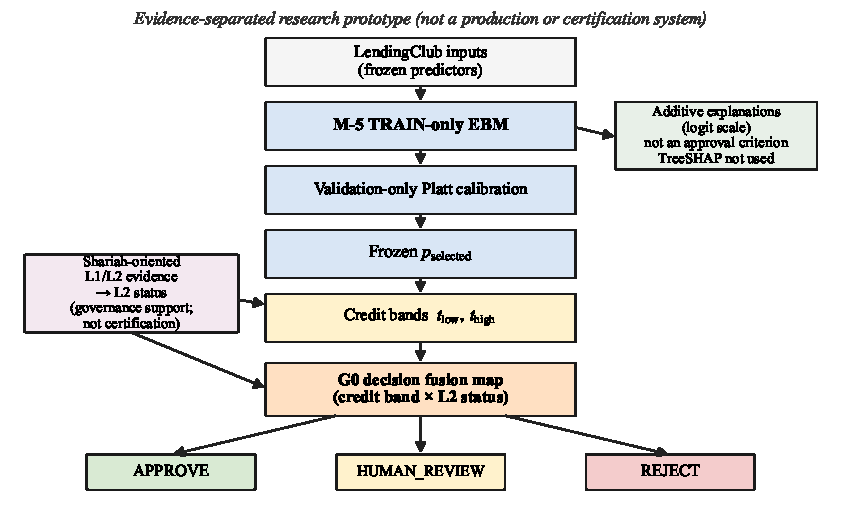
\includegraphics[width=\textwidth]{fig1_architecture.pdf}
\caption{Evaluated evidence-separated research-prototype architecture. Center path: LendingClub inputs \(\rightarrow\) M-5 TRAIN-only EBM \(\rightarrow\) validation-only Platt \(\rightarrow\) frozen \(p_{\mathrm{selected}}\) \(\rightarrow\) credit bands \(\rightarrow\) G0 fusion \(\rightarrow\) \texttt{\{APPROVE, HUMAN\_REVIEW, REJECT\}}. Right path: additive logit-scale explanations (not an approval criterion; TreeSHAP not used). Left path: Shariah-oriented L1/L2 evidence to L2 status (governance support, not certification). No fraud-detection layer was evaluated. This is not a production deployment.}
\label{fig:arch}
\end{figure*}

The system is a research prototype for Shariah-oriented governance and evidence traceability. It is decision-support / evidence-gap handling. It does not replace a Shariah Board.

\subsection{LendingClub Dataset}

The primary executed dataset is the LendingClub granting-model extract \sha{LC_loans_granting_model_dataset.csv}, Zenodo DOI \texttt{10.5281/zenodo.11295916}, version 0.1, license CC-BY-4.0 \cite{b20}. Official Zenodo creators are M. J. Ariza-Garz\'on, M. Sanz-Guerrero, and J. Arroyo Gallardo (Lending Club listed as data collector) \cite{b20}. File SHA-256 is \sha{207d65b2712f775a91404496ab27c786ac0da6b0f977f849e6d5d8149e925acc}. The extract contains 1,347,681 rows \(\times\) 15 columns.

The extract is depositor-filtered from a parent Kaggle Lending Club file. Kaggle is not a third executed dataset. The file contains originated-and-resolved loans; rejected applicants are absent (selection bias). The extract is recorded as US P2P 2007--2018. It is \textbf{not} Islamic-finance data and does \textbf{not} contain contract-level Shariah evidence fields sufficient for applicant-level Shariah compliance determination.

Target column: \texttt{Default}. Freeze coding: \texttt{1} = Charged Off, \texttt{0} = Fully Paid. A Zenodo target-documentation conflict was recorded; the freeze coding controls.

Time index used for splitting: \texttt{issue\_month} derived from \texttt{issue\_d}. Split hashes:

\begin{itemize}
\item TRAIN \(n=941267\), hash \sha{02ba5877fdf189ba807a6b8e4463383fd04e86f6b3a65a1a5e9583f8b2d989d2}
\item VALIDATION \(n=197528\), hash \sha{d1585d22e101c717bf52426e8e625da960c975aa35db703a435bc4a7f8b3df91}
\item TEST \(n=208886\), hash \sha{4dfedb1ad7785fa3833047135b1883676f3e1b49aca9c87fcdb346e64fd489c6}

\end{itemize}
Prevalence differences by split (train 18.7\%, validation 24.9\%, test 21.2\%) are descriptive context; M-5 TEST stored prevalence is \(0.2117901630554465\) with \(n_{\text{positive}}=44240\).

\subsection{UCI Credit Card Default Dataset}

The independent secondary dataset is UCI Default of Credit Card Clients, UCI dataset 350, DOI \texttt{10.24432/C55S3H} \cite{b4}, \cite{b21}. Zip SHA-256: \sha{56c885f84457f6680f8438f02bfcdac9579323d8a94465ee5f26e32baa727602}. The table has 30,000 rows \(\times\) 25 columns. Target: \texttt{default payment next month} (\texttt{1} = default next month). The UCI target is \textbf{not} equivalent to the LendingClub charged-off / fully-paid coding.

UCI has no calendar timestamps. Split: stratified 70/15/15 by target, seed 42:

\begin{itemize}
\item TRAIN \(n=20{,}999\), hash \sha{70b1819de66fdae6793691e83224b5dc4e1956c021b582ffcf0a89791c9ac2f1}
\item VALIDATION \(n=4{,}499\), hash \sha{76a91b4b6fefbfd111d6a7c536ad222330c3bcf0f4358c259e40d4814382bcd4}
\item TEST \(n=4{,}502\), hash \sha{0783db42ac57a277f79379e0a62ef00f2a2b189f868ed993cebdf16def404126}

\end{itemize}
The tables were not merged. Undocumented UCI codes remain unlabeled. UCI analysis does not implement the Shariah governance layer and does not validate the LendingClub architecture. German Credit \cite{b22} and Australian Credit Approval \cite{b23} remain literature-context benchmarks only and were not executed.

\setcounter{table}{0}
\begin{table*}[!t]
\caption{Executed datasets (literature-only German Credit and Australian Credit Approval are excluded).}
\label{tab:t1}
\setlength{\tabcolsep}{3pt}
\centering
\footnotesize
\begin{tabularx}{\linewidth}{|>{\raggedright\arraybackslash}p{0.16\linewidth}|>{\raggedright\arraybackslash}X|>{\raggedright\arraybackslash}X|}
\hline
Field & LendingClub granting-model extract & UCI Default of Credit Card Clients \\
\hline
Role & \textbf{PRIMARY} credit-risk / decision-architecture setting & \textbf{Independent} credit-risk / calibration methodology only \\
\hline
Source & Zenodo DOI \texttt{10.5281/zenodo.11295916}; CC-BY-4.0; version 0.1 \cite{b20} & UCI dataset 350; DOI \texttt{10.24432/C55S3H} \cite{b4}, \cite{b21} \\
\hline
Characterization & US P2P 2007--2018; not an Islamic-finance sample; originated-and-resolved loans, not the full application funnel & 2005 Taiwan credit-card snapshot; no calendar timestamps \\
\hline
Full-file size & 1,347,681 \(\times\) 15 & 30,000 \(\times\) 25 \\
\hline
File / zip SHA-256 & \sha{207d65b2712f775a91404496ab27c786ac0da6b0f977f849e6d5d8149e925acc} & \sha{56c885f84457f6680f8438f02bfcdac9579323d8a94465ee5f26e32baa727602} \\
\hline
Target & \texttt{Default} (1 = Charged Off, 0 = Fully Paid) & \texttt{default payment next month} (1 = default next month) \\
\hline
Split & Temporal by \texttt{issue\_month}: TRAIN \(\le\) 2016-03; VAL 2016-04--2017-01; TEST \(\ge\) 2017-02 & Stratified 70/15/15 by target, seed 42 \\
\hline
TRAIN / VAL / TEST \(n\) & 941,267 / 197,528 / 208,886 & 20,999 / 4,499 / 4,502 \\
\hline
TEST hash & \sha{4dfedb1ad7785fa3833047135b1883676f3e1b49aca9c87fcdb346e64fd489c6} & \sha{0783db42ac57a277f79379e0a62ef00f2a2b189f868ed993cebdf16def404126} \\
\hline
Merged? & Not merged with UCI & Not merged with LendingClub \\
\hline
Shariah contract-level fields & None sufficient for applicant-level determination & Governance layer not applied \\
\hline
\end{tabularx}
\end{table*}

\subsection{Feature Policy and Leakage Controls}

LendingClub primary predictors (both LC EBMs): \texttt{revenue}, \texttt{dti\_n}, \texttt{loan\_amnt}, \texttt{fico\_n}, \texttt{emp\_length}, \texttt{purpose}, \texttt{home\_ownership\_n}, \texttt{addr\_state}, \texttt{zip\_code}.

Excluded from the primary credit model: \texttt{id}, \texttt{issue\_d}, \texttt{experience\_c}, \texttt{title}, \texttt{desc}. Free-text \texttt{title} and \texttt{desc} were retained as a possible future branch; \textbf{no text model was built}. \texttt{addr\_state} and \texttt{zip\_code} are quasi-identifiers.

The LendingClub preprocessor for the downstream pipeline is fit on TRAIN only (\sha{lendingclub_preprocessor.joblib}). High-cardinality \texttt{zip\_code} is one-hot encoded for families that consume the expanded matrix (logistic regression, random forest, XGBoost). The EBM uses the nine imputed native columns rather than the one-hot expansion, because one-hot encoding would destroy additive per-original-feature structure. \texttt{dti\_n==999} is unlabeled. Newly discovered leakage, beyond frozen exclusions, is recorded as none.

UCI retained columns are the standard LIMIT\_BAL / demographics / PAY\_\emph{ / BILL\_AMT} / PAY\_AMT* block; \texttt{ID} is excluded.

Credit features are excluded from the Shariah evidence object (evidence firewall). \texttt{purpose} is not mapped to a Murabaha, Ijarah, or other contract type (purpose-invariance).

\subsection{Temporal Train/Validation/Test Design}

LendingClub is split \textbf{temporally} by \texttt{issue\_month}:

\begin{itemize}
\item TRAIN: \texttt{issue\_month <= 2016-03}
\item VALIDATION: \texttt{2016-04} through \texttt{2017-01}
\item TEST: \texttt{issue\_month >= 2017-02}

\end{itemize}
Hash method: SHA-256 of sorted \texttt{issue\_month} and \texttt{id} lines within each split.

UCI cannot use a calendar split. It uses a stratified random split with seed 42, documented as such. UCI therefore cannot support a temporal-generalization claim of the LendingClub type.

TEST is reporting-only after freeze for LendingClub family metrics (M-4B), calibration reporting (M-5), and decision counts on stored \texttt{p\_selected}. Thresholds and calibrators were identified on validation. TEST was not used to choose the M-4B family, the Platt calibrator, or \(t_{\text{low}}\) / \(t_{\text{high}}\) / \(t^{*}\).

\subsection{Baseline Models (M-4B)}

\textbf{M-4B} compares four families on LendingClub. Hyperparameters were frozen before TEST. Validation seeds: 42, 123, 2024, 3407, 9999. Final TEST seed: 42.

Recorded configurations (seed-42 test \texttt{config} blocks):

\begin{sloppypar}
\begin{itemize}
\item \textbf{Logistic regression:} \texttt{liblinear}, L2, \(C=1.0\), \texttt{class\_weight='balanced'}, \texttt{max\_iter=300}. StandardScaler on the numeric block, fit on the current training matrix.
\item \textbf{Random forest:} 80 trees, \texttt{max\_depth=12}, \texttt{min\_samples\_leaf=100}, \texttt{max\_features='sqrt'}, \texttt{class\_weight='balanced'}, sparse CSC input.
\item \textbf{XGBoost (LendingClub only):} \texttt{binary:logistic}, 300 estimators, learning rate 0.05, \texttt{max\_depth=4}, \texttt{min\_child\_weight=20}, subsample 0.8, \texttt{colsample\_bytree=0.8}, \texttt{scale\_pos\_weight} computed on fitting labels (train+validation refit 4.061108666764441). Early stopping used validation during the train/val phase only; not used on TEST. This is \textbf{not} M-9.4-X.
\item \textbf{EBM:} InterpretML EBM, \texttt{interactions=0}, \texttt{max\_bins=256}, learning rate 0.02, \texttt{max\_rounds=200}, \texttt{outer\_bags=4}, nine native columns. No class-weight argument in EBM 0.7.8.

\end{itemize}
\end{sloppypar}
Primary validation criterion: mean PR-AUC across the five seeds. Best mean validation PR-AUC is 0.388473. Candidates within 0.005: EBM and XGBoost. Among those, lowest mean Brier then simplicity selected \textbf{EBM} (mean validation PR-AUC \(=0.385841\), Brier \(=0.179907\)). TEST numbers were not used to choose the family. All completed families were still refit on TRAIN+VALIDATION and evaluated once on TEST after freeze.

The selected M-4B EBM dump path is \sha{results/artifacts/final_explainable_boosting_machine_seed42.joblib}. Its SHA-256 is \textbf{not recorded}. That model is \textbf{not} used from the decision-fusion stage onward.

\subsection{Train-only EBM and Calibration (M-5)}

\textbf{M-5} retrains an EBM on TRAIN only (\texttt{n\_train=941267}) with frozen M-4B hyperparameters. Artifact: \sha{results/calibration/artifacts/ebm_train_only_seed42.joblib}, SHA-256 \sha{8d373df1b576ca74f498d2bfcc54653cbf43d37b0af69400a26e20ab98a3a0c4}. Preprocessor: \sha{lendingclub_preprocessor.joblib} (train-only), not the M-4B train+validation preprocessor.

Protocol: validation-only calibration, no train+validation calibrator refit. Candidates stored: raw, Platt, isotonic. Calibrators are fit on VALIDATION raw probabilities and labels only. They are \textbf{not} fit on TEST and \textbf{not} refit on TRAIN+VALIDATION.

Platt scaling \cite{b14} maps raw scores by
\begin{equation}
\label{eq:platt}
p_{\mathrm{platt}}
=
\sigma\bigl(a \cdot \operatorname{logit}(p_{\mathrm{raw}}) + b\bigr).
\end{equation}
where \(\sigma\) is the logistic sigmoid, \(a\) and \(b\) are fit by unregularized logistic regression (\texttt{C=}\(\infty\), solver \texttt{lbfgs}) on \(\operatorname{logit}(p_{\mathrm{raw}})\), and frozen parameters are \(a = 1.1988263209549705\), \(b = 0.6697765046966161\), and \texttt{fit\_split = validation}.
Isotonic regression is stored (\texttt{y\_min=0}, \texttt{y\_max=1}, increasing, \texttt{out\_of\_bounds='clip'}) and is \textbf{not} selected \cite{b16}.

Selection rule: validation Brier; 0.001 practical tie; simplicity order \texttt{raw > platt > isotonic}; declared before test. Best validation Brier is 0.17469431274375435 (isotonic). Platt validation Brier is 0.1748453678205707, within 0.001 of isotonic, so \textbf{Platt} is selected. All five validation seeds selected Platt.

TEST calibrated vector: \sha{results/calibration/test/ebm_seed42_calibrated.csv}, SHA-256 \sha{e15ddd2f85a6c3fc9d0a79eecb578f7a94ded8a7efc63d9d114212728b2469eb}. Column \texttt{p\_selected} equals \texttt{p\_platt} from \eqref{eq:platt}. Decision fusion and later analyses consume this stored vector. ECE uses 10 equal-width bins on \([0,1]\); empty bins are excluded from ECE and maximum calibration error (MCE).

Platt is a strictly increasing map of \(p_{\mathrm{raw}}\). Stored TEST ROC-AUC and PR-AUC of Platt therefore equal stored raw. Calibration is not claimed to improve discrimination.

Reliability-diagram image files named in the calibration report are \textbf{not retained} in the repository and are omitted from this manuscript. They are not regenerated from scores.

\subsection{Explainability}

The explainable reference is the additive M-5 EBM (\texttt{interactions=0}). Method:

\begin{itemize}
\item Exact additive interventional SHAP-style decomposition on the logit / \texttt{decision\_function} scale:
\begin{equation}
\label{eq:shap}
\phi_i(x) = g_i(x_i) - \operatorname{mean}_{\mathrm{TRAIN}} g_i.
\end{equation}
\item TreeSHAP was \textbf{not} used; it is not mathematically appropriate for this first-order GAM \cite{b13}.
\item \texttt{shap.AdditiveExplainer} was not used (masker / mixed categoricals).
\item Platt is not inside the explanation.
\item Sample: 5,000 TEST rows, \texttt{RandomState(42)}, without replacement; labels not used to draw the sample. Not the full TEST set.

\end{itemize}
In \eqref{eq:shap}, \(g_i\) is the fitted additive EBM term for feature \(i\), and the mean is taken over TRAIN. The EBM is a transparent-model \textbf{reference}, not ground truth, not causal, and not an approval criterion \cite{b12}. Perfect rank agreement between SHAP and centered EBM terms is the identity of those centered terms, not independent confirmation from a second model class.

\textbf{Documented provenance limitation (not silently rewritten):} an explainability-report opening sentence refers to ``the frozen Stage 4B model.'' Metadata (\texttt{model\_id=ebm\_train\_only\_seed42}; \sha{stage5_model_path=results/calibration/artifacts/ebm_train_only_seed42.joblib}) identify the TRAIN-only M-5 EBM, not \sha{results/artifacts/final_explainable_boosting_machine_seed42.joblib}. This paper follows the metadata.

\subsection{Shariah-Oriented Governance Layer}

\textbf{Required description:} research prototype for Shariah-oriented governance and evidence traceability. Not certification \cite{b27}. Not a fatwa. Not an automated Shariah-compliance verdict. Not expert-validated Shariah decisioning (\texttt{EXPERT\_VALIDATED} = none).

\begin{center}
\footnotesize
\setlength{\tabcolsep}{3pt}
\begin{tabularx}{\columnwidth}{|>{\raggedright\arraybackslash}p{0.28\columnwidth}|>{\raggedright\arraybackslash}X|}
\hline
Layer & Treatment in this study \\
\hline
A. Verified source / provenance & SBP SGF 2025 via IFPD Circular 08 of 2024 \cite{b24}, \cite{b25}; SBP IBD Circular 01 of 2012 \cite{b26}; SECP SGR 2023 Regulation 7 \cite{b27}; AAOIFI SS 8 / SS 9 \textbf{identity} only \cite{b28}, \cite{b29}; AAOIFI GS listing \cite{b30}; IFSB-10 identity/FAQ \cite{b31} \\
\hline
B. Implemented predicates & L1 dataset readiness vs L2 per-application evaluation; source-mapped SBP/SECP rules at \sha{SOURCE_VERIFIED_PENDING_EXPERT_REVIEW}; AAOIFI identity/unavailability gates only; credit-feature firewall; purpose-invariance \\
\hline
C. Evidence / schema gaps & L1 \sha{INSUFFICIENT_SCHEMA_FOR_APPLICANT_DETERMINATION}; L2 \texttt{INSUFFICIENT\_INFORMATION} on all LC TEST rows; AAOIFI possession \texttt{NOT\_VERIFIED}; one unsupported retired rule \\
\hline
D. Unvalidated / unavailable & AAOIFI operative clauses not retrieved or implemented; no \texttt{EXPERT\_VALIDATED} rule \\
\hline
\end{tabularx}
\end{center}

The fused \texttt{INSUFFICIENT\_INFORMATION} result is an evidence/schema limitation. LendingClub does not contain invoices, possession records, or other contract-level Shariah fields contemplated by Murabaha documentary circulars \cite{b26}. \texttt{INSUFFICIENT\_INFORMATION} is \textbf{not} a finding that an applicant is Shariah non-compliant, that a contract is compliant or non-compliant, or that the ML score determines Shariah compliance. The ML score does not determine Shariah compliance. Human review is not certification.

\subsection{Decision Policies}

Thresholds were identified on validation under a researcher cost scenario, not operational cost:

\begin{itemize}
\item FN:FP \(= 5:1\), \(C_{\text{REVIEW}} = 0.25 \times C_{\text{FP}}\)
\item Two-threshold credit bands: \(t_{\text{low}}=0.06\), \(t_{\text{high}}=0.69\)
\item Monolithic single threshold: \(t^{*}=0.16\)

\end{itemize}
Fig.~\ref{fig:policy} diagrams these frozen validation-derived thresholds. No new grid was searched at fusion time. Credit bands on stored \(p_{\mathrm{selected}}\) follow
\begin{equation}
\label{eq:bands}
\operatorname{band}(p)
=
\begin{cases}
\mathrm{LOW}, & p < t_{\mathrm{low}},\\
\mathrm{HIGH}, & p \ge t_{\mathrm{high}},\\
\mathrm{MEDIUM}, & \text{otherwise}.
\end{cases}
\end{equation}
with the frozen identification \(t_{\mathrm{low}}=0.06\) and \(t_{\mathrm{high}}=0.69\).

\begin{figure*}[!t]
\centering
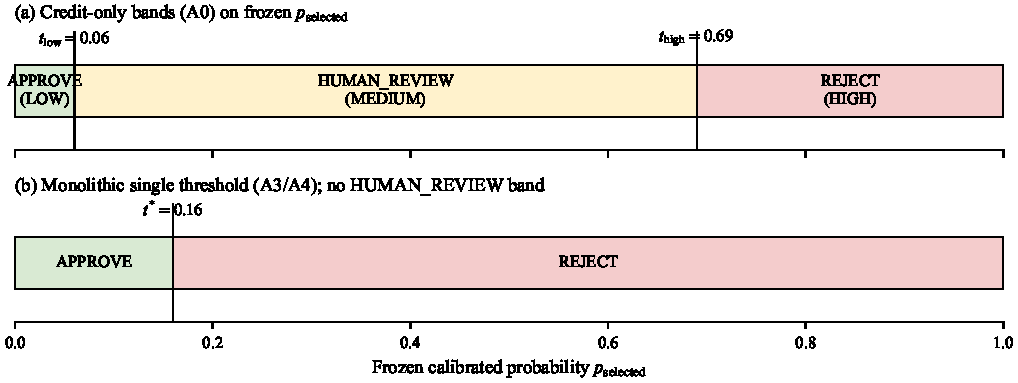
\includegraphics[width=0.92\textwidth]{fig3_decision_policy_thresholds.pdf}
\caption{Frozen research decision thresholds on \(p_{\text{selected}}\) (transcribed from \texttt{results/decision/v2/frozen\_policy.json}). Panel (a): credit-only bands A0 with \(t_{\text{low}}=0.06\) and \(t_{\text{high}}=0.69\). Panel (b): monolithic A3/A4 with \(t^{*}=0.16\). \texttt{HUMAN\_REVIEW} is a simulated research-policy band, not a collected human-review outcome and not a real loan-origination result. Fused map A1 applies the same credit bands through the G0 matrix (Table~\ref{tab:t9}).}
\label{fig:policy}
\end{figure*}

\setcounter{table}{8}
\begin{table}[!t]
\caption{G0 fusion matrix. \texttt{INSUFFICIENT\_INFORMATION} is not converted to \texttt{PASS} or to religious non-compliance. The same matrix is not repeated as a separate figure.}
\label{tab:t9}
\setlength{\tabcolsep}{2.5pt}
\centering
\scriptsize
\begin{tabularx}{\columnwidth}{|>{\raggedright\arraybackslash}X|c|c|c|}
\hline
Governance (L2) & LOW & MEDIUM & HIGH \\
\hline
{\ttfamily NOT\_STRUCTURABLE\_\allowbreak WITHOUT\_\allowbreak REDESIGN} & REJECT & REJECT & REJECT \\
\hline
{\ttfamily INSUFFICIENT\_\allowbreak INFORMATION} & HUMAN\_REVIEW & HUMAN\_REVIEW & REJECT \\
\hline
\texttt{REVIEW} & HUMAN\_REVIEW & HUMAN\_REVIEW & REJECT \\
\hline
\texttt{PASS} & APPROVE & HUMAN\_REVIEW & REJECT \\
\hline
\end{tabularx}
\end{table}


L1 schema status is dataset context and is \textbf{not} the G0 matrix input. L2 \texttt{overall\_governance\_status} is the matrix input.

Named maps (A3 identical to A4):

\begin{itemize}
\item \textbf{A0} \texttt{credit\_only\_selected\_bands}: credit bands only.
\item \textbf{A1} \texttt{fused\_evidence\_separated\_v2}: G0 fusion.
\item \textbf{A3/A4} \texttt{monolithic\_credit\_threshold}: single threshold \(t^{*}\) with no review band.

\end{itemize}
These are policy analyses on frozen \texttt{p\_selected}, not real-world approval performance. Maps are not ranked as best / optimal / winner.

Recorded freeze SHA-256 values: v2 \sha{b874782326a8f20ed9bb7df1aa5ed1c75f883d8b6cba76b68991181d50b1604b}; v1 \sha{4d3da6a9e5bac2b38b546c7a5a60e870bf83f30adcadf67f067f99951e32f0c4}; decision-count table \sha{90759eb72f1173b40b5b9363c21b0ef3d6f1cde5042748eb57871d49fb73d5ee}.


\section{Experimental Protocol}

The empirical program is sequential and frozen. Later analyses do not retune thresholds, refit calibration, or reopen family selection.

\begin{center}
\footnotesize
\setlength{\tabcolsep}{2.5pt}
\begin{tabularx}{\columnwidth}{|>{\raggedright\arraybackslash}p{0.16\columnwidth}|>{\raggedright\arraybackslash}X|>{\raggedright\arraybackslash}p{0.20\columnwidth}|>{\raggedright\arraybackslash}X|}
\hline
Stage & What was frozen & Test-set role & Authorization class for later citation \\
\hline
Data / split & Acquisition, hashes, feature policy, splits & Split construction & Data provenance \\
\hline
Preprocessing & Train-only LC preprocessor & Not a predictor test & Methodology \\
\hline
M-4B & Four-family LC models; EBM selected on validation & One family test after TRAIN+VAL refit & Family test after freeze \\
\hline
M-5 & TRAIN-only EBM; validation-only calibrator selection & Reporting of raw/Platt/isotonic & M-5 pipeline reporting \\
\hline
Explainability & Attributions of M-5 EBM & Descriptive sample \(n=5000\) & Descriptive of that model \\
\hline
Governance & L1/L2 predicates & Governance evidence, not certification & Prototype governance \\
\hline
Thresholds & Identification on validation & None for new search & Freeze-backed identification \\
\hline
Fusion & G0 fusion on stored \texttt{p\_selected} & Decision counts & Freeze-backed policy counts \\
\hline
Map ablation & Ablation of frozen maps & Previously exposed test set & Class B documentation-gap authorization \\
\hline
Cost sensitivity & Assumed-\(r\) cost sensitivity & Stored counts under alternative \(r\) & Class C exploratory \\
\hline
Hypothetical G1/G3 & Hypothetical allocation & Hypothetical allocation & Class C exploratory; not Shariah findings \\
\hline
UCI LR+EBM & UCI-local family test & UCI test & Approved independent methodology (\textbf{M-9.4-AE}) \\
\hline
UCI XGBoost & Execution-time UCI family expansion & UCI test & Class C \texttt{DEVIATION-001}; \textbf{M-9.4-X} exploratory \\
\hline
Integrity check & Hash / identity check & No new scores & Integrity; not confirmatory science \\
\hline
Year mix & 2017/2018 mix of frozen maps & Post-hoc slices & Exploratory / descriptive post-hoc \\
\hline
Evidence-gap algebra & Algebra of A1 review & Existing L2 statuses & Analysis-only; not Shariah validation \\
\hline
Side-by-side citation & Citation comparison LC vs UCI & No new AUC & Analysis-only \\
\hline
\end{tabularx}
\end{center}

M-4B and M-5 test confidence intervals are percentile bootstrap, 1000 row resamples, seed 42, not used for tuning. UCI XGBoost remains exploratory under \texttt{DEVIATION-001} and is not a primary validated model. Metric wrappers used in the stored artifacts are ROC-AUC = \texttt{sklearn.metrics.roc\_auc\_score}, with PR-AUC, Brier, and log loss as recorded in the project metric-definition notes.


\section{Results}

Every numeral below is transcribed from a stored artifact. No new test metric is computed in this manuscript.

\subsection{LendingClub Baseline Results}

Context: \textbf{M-4B}. TEST \(n=208{,}886\). TRAIN+VALIDATION refit after family freeze. These metrics are \textbf{not} the downstream decision scores.

\setcounter{table}{1}
\begin{table*}[!t]
\caption{Two LendingClub EBMs (must not be collapsed).}
\label{tab:t2}
\setlength{\tabcolsep}{3pt}
\centering
\footnotesize
\begin{tabularx}{\linewidth}{|>{\raggedright\arraybackslash}p{0.18\linewidth}|>{\raggedright\arraybackslash}X|>{\raggedright\arraybackslash}X|}
\hline
 & M-4B TEST EBM & M-5 raw / Platt TEST \\
\hline
Training split & TRAIN+VALIDATION refit & TRAIN only (\texttt{n\_train=941267}) \\
\hline
Preprocessor & \sha{preprocessor_train_plus_validation.joblib} & \sha{lendingclub_preprocessor.joblib} \\
\hline
Model dump & \sha{results/artifacts/final_explainable_boosting_machine_seed42.joblib} (SHA-256 \textbf{not recorded}) & \sha{results/calibration/artifacts/ebm_train_only_seed42.joblib} (SHA-256 \sha{8d373df1b576ca74f498d2bfcc54653cbf43d37b0af69400a26e20ab98a3a0c4}) \\
\hline
TEST \(n\) & 208,886 & 208,886 (same chronological test split) \\
\hline
ROC-AUC & \textbf{0.6799408767429772} & \textbf{0.6776693941139847} \\
\hline
Gap classification & \textbf{EXPLAINED} (different fitted models) & Same \\
\hline
Used from decision fusion onward & \textbf{No} & \textbf{Yes} (\texttt{p\_selected}) \\
\hline
\end{tabularx}
\end{table*}


The gap is not a calibration effect on rank: M-5 Platt TEST ROC-AUC equals stored raw. It is not an unresolved error.

\setcounter{table}{2}
\begin{table*}[!t]
\caption{M-4B LendingClub TEST metrics (seed 42; TRAIN+VALIDATION refit).}
\label{tab:t3}
\centering
\footnotesize
\setlength{\tabcolsep}{3.5pt}
\renewcommand{\arraystretch}{1.2}
\begin{tabular}{|l|c|c|c|c|}
\hline
Family & ROC-AUC & PR-AUC & Brier & Log loss \\
\hline
\texttt{logistic\_regression} & 0.6763559009686606 & 0.3406477564928828 & 0.21998431914321218 & 0.6354126164492524 \\
\hline
\texttt{random\_forest} & 0.6609260816246479 & 0.33258566142201473 & 0.23597628092130948 & 0.6648999360582141 \\
\hline
\texttt{xgboost} (LC only) & 0.6854404067747387 & 0.3576696570242051 & 0.2136380371614269 & 0.6149464126269267 \\
\hline
\texttt{explainable\_boosting\_machine} & 0.6799408767429772 & 0.3534066581608194 & 0.15684495750106664 & 0.48493888407781477 \\
\hline
\end{tabular}
\end{table*}


Percentile 95\% bootstrap CIs are stored with the same metrics (1000 resamples). For the selected EBM: ROC-AUC CI \([0.6772520975812178, 0.6828319764466856]\); PR-AUC CI \([0.3492795049814313, 0.3577134296795478]\); Brier CI \([0.15586719460814155, 0.1579539606709722]\).

ECE is \textbf{not stored} for Stage 4B logistic regression, nor for the other Stage 4B families (random forest, XGBoost, EBM), in the Stage 4B test-metric artifact. No Stage 4B ECE value is calculated or inferred here.

TEST PR-AUC is lower than validation PR-AUC for every family. Descriptive year slices of the M-4B TEST EBM (not used to retune): 2017 ROC-AUC 0.677804, PR-AUC 0.377247, Brier 0.168236; 2018 ROC-AUC 0.675593, PR-AUC 0.276294, Brier 0.125866.

M-4B LC XGBoost TEST ROC-AUC \(0.6854404067747387\) is a Stage 4B family result. It is not the decision-fusion model and is not M-9.4-X.

Fig.~\ref{fig:roc} plots the stored TEST ROC-AUC values for the four M-4B families and the distinct M-5 TRAIN-only EBM (raw and Platt ROC-AUC are identical). The figure does not collapse the two EBM fits.

\begin{figure*}[!t]
\centering
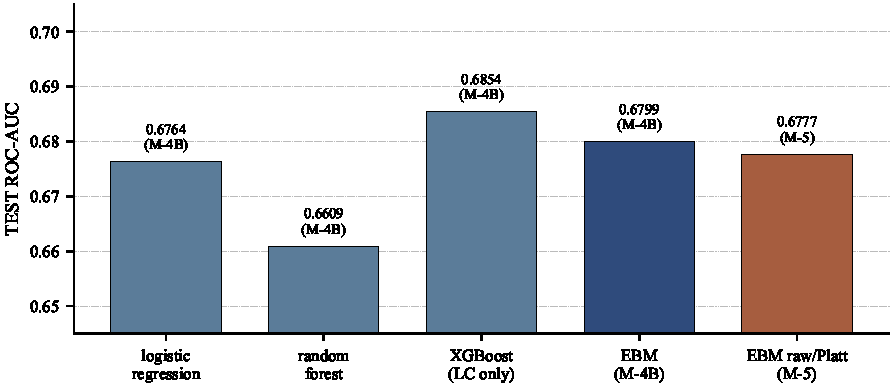
\includegraphics[width=0.92\textwidth]{fig2_model_test_roc_auc.pdf}
\caption{Stored LendingClub TEST ROC-AUC values. The first four bars are context \textbf{M-4B} (TRAIN+VALIDATION refit family TEST; seed 42). The fifth bar is context \textbf{M-5} (TRAIN-only EBM; Platt and raw ROC-AUC both equal \(0.6776693941139847\)). Values are transcribed from \texttt{results/metrics/stage4b\_test\_metrics.json} and \texttt{results/calibration/metrics/stage5\_test\_metrics.json}. M-4B and M-5 are different fitted models and must not be averaged.}
\label{fig:roc}
\end{figure*}

\subsection{Calibration Results}

Context: \textbf{M-5}. TEST \(n=208{,}886\); \(n_{\text{positive}}=44240\); prevalence \(0.2117901630554465\).

\setcounter{table}{3}
\begin{table*}[!t]
\caption{M-5 calibration metrics (TRAIN-only EBM; calibrators fit on validation only).}
\label{tab:t4}
\centering
\scriptsize
\setlength{\tabcolsep}{1.8pt}
\renewcommand{\arraystretch}{1.12}
\textbf{(a)} Validation (\(n=197{,}528\); \(n_{\mathrm{positive}}=49163\); prevalence \(0.24889129642379815\)).\\[0.6mm]
\resizebox{\linewidth}{!}{%
\begin{tabular}{|l|c|c|c|c|c|c|}
\hline
Method & Brier & Log loss & ECE & MCE & ROC-AUC & PR-AUC \\
\hline
raw & 0.17990848215908947 & 0.5412792598426245 & 0.06286213537136044 & 0.6023420058578064 & 0.6656900641018727 & 0.38583491323890046 \\
\hline
Platt (selected) & 0.1748453678205707 & 0.5278455947278384 & 0.0022124994740890247 & 0.02643192035246955 & 0.6656900641018727 & 0.38583491323890046 \\
\hline
isotonic (not selected) & 0.17469431274375435 & 0.5273917354891987 & \(1.596976975349043\times 10^{-17}\) & \(1.1102230246251565\times 10^{-16}\) & 0.6661439550959414 & 0.3823621419016197 \\
\hline
\end{tabular}%
}\\[2.2mm]
\textbf{(b)} TEST (reporting only).\\[0.6mm]
\resizebox{\linewidth}{!}{%
\begin{tabular}{|l|c|c|c|c|c|c|}
\hline
Method & Brier & Log loss & ECE & MCE & ROC-AUC & PR-AUC \\
\hline
raw & 0.1579357158246714 & 0.4880855738039092 & 0.03753450535939786 & 0.38427225714072644 & 0.6776693941139847 & 0.35096314719303284 \\
\hline
Platt (selected) & 0.15616920271522994 & 0.48357015583149326 & 0.020267295489117824 & 0.1869468566677409 & 0.6776693941139847 & 0.35096314719303284 \\
\hline
isotonic (not selected) & 0.1561969364282068 & 0.48360807473639705 & 0.020046149884935992 & 0.30756843800322053 & 0.6775144297473418 & 0.3462755761696744 \\
\hline
\end{tabular}%
}
\end{table*}

Platt TEST ROC-AUC equals raw. Isotonic is piecewise constant and slightly changes TEST ranking (PR-AUC \(0.35096314719303284\) \(\rightarrow\) \(0.3462755761696744\)).

Paired TEST differences (calibrated - raw), not recomputed: Platt Brier \(-0.001767\) (bootstrap CI \([-0.002005, -0.001508]\)); Platt ECE \(-0.017267\) (CI \([-0.020730, -0.014170]\)). Intervals are not interpreted as hypothesis-test \(p\)-values in the source record.

Descriptive temporal slices under frozen Platt (not a new confirmatory test): 2017 \(n=152726\), Platt ECE \(0.005096425775164428\); 2018 \(n=56160\), Platt ECE \(0.06152417312325683\). On 2018, Platt increases Brier, log loss, and ECE relative to raw. The validation window is 2016-04 through 2017-01; this is classified as temporal transfer failure, not a reason to recode the frozen calibrator.

Reliability diagrams named in the calibration report (10 equal-width ECE bins) are historical path references. Those image files are not retained and are not regenerated from scores. Fig.~\ref{fig:cal} instead plots the \textbf{stored} TEST risk-range table (\texttt{results/calibration/\allowbreak tables/\allowbreak stage5\_risk\_ranges.csv}): mean predicted probability versus observed default rate for raw and selected Platt. That table uses the five stored ranges \(0.00\)--\(0.10\), \(0.10\)--\(0.20\), \(0.20\)--\(0.30\), \(0.30\)--\(0.50\), and \(0.50\)--\(1.00\); it is not a reconstruction of the omitted 10-bin ECE reliability image.

\begin{figure}[!t]
\centering
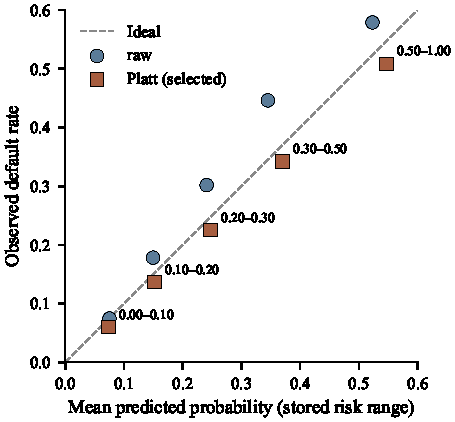
\includegraphics[width=\columnwidth]{fig5_calibration_risk_ranges.pdf}
\caption{Stored TEST risk-range calibration for the M-5 EBM: mean predicted probability versus observed default rate for raw and Platt (selected), transcribed from \texttt{stage5\_risk\_ranges.csv}. Dashed line: ideal equality. Labels mark the Platt range intervals. This is not the omitted 10-bin ECE reliability diagram and does not recompute ECE.}
\label{fig:cal}
\end{figure}

\subsection{Explainability Results}

Context: M-5 EBM; descriptive attributions; sample \(n=5000\).

\setcounter{table}{4}
\begin{table*}[!t]
\caption{Global mean absolute attribution (logit scale; sample of 5,000 TEST rows).}
\label{tab:t5}
\renewcommand{\arraystretch}{1.22}
\footnotesize
\begin{tabularx}{\linewidth}{|>{\raggedright\arraybackslash}X|c|c|c|c|}
\hline
Feature & shap\_mean\_abs & shap\_rank & ebm\_mean\_abs & ebm\_rank \\
\hline
\texttt{fico\_n} & 0.3072104502059198 & 1 & 0.3072104502059198 & 1 \\
\hline
\texttt{loan\_amnt} & 0.2887712351465414 & 2 & 0.2887712351465414 & 2 \\
\hline
\texttt{dti\_n} & 0.15084749758493932 & 3 & 0.15084749758493932 & 3 \\
\hline
\texttt{revenue} & 0.1449737450602624 & 4 & 0.14497374506026237 & 4 \\
\hline
\texttt{home\_ownership\_n} & 0.12252891641707762 & 5 & 0.12252891641707761 & 5 \\
\hline
\texttt{zip\_code} & 0.11979470116252551 & 6 & 0.11979470116252551 & 6 \\
\hline
\texttt{purpose} & 0.10257411348554467 & 7 & 0.10257411348554467 & 7 \\
\hline
\texttt{emp\_length} & 0.03984046466379107 & 8 & 0.03984046466379107 & 8 \\
\hline
\texttt{addr\_state} & 0.007289702255172925 & 9 & 0.007289702255172925 & 9 \\
\hline
\end{tabularx}
\end{table*}


Agreement: \texttt{overlap\_top3=1.0}, \texttt{overlap\_top5=1.0}, \texttt{overlap\_top9=1.0}, Spearman \(=1.0\), Kendall \(=1.0\), \texttt{additive\_reconstruction\_max\_abs\_error} \(=8.881784197001252\times 10^{-16}\). This identity is expected for centered additive terms. It is not independent confirmation from a second model class and is not a causal ranking of default drivers. Fig.~\ref{fig:attr} visualizes the same stored mean-absolute series.

\begin{figure}[!t]
\centering
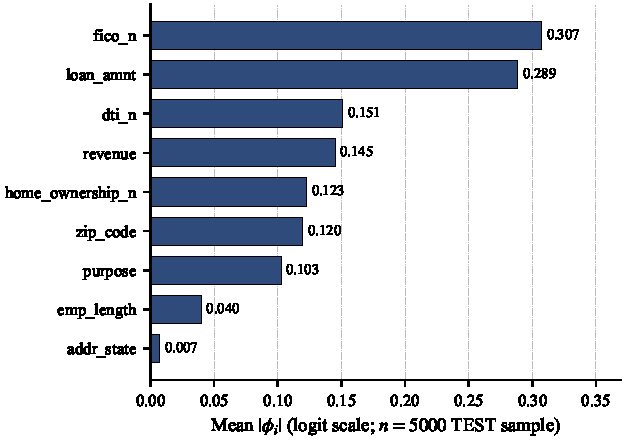
\includegraphics[width=\columnwidth]{fig4_global_attribution.pdf}
\caption{Global mean absolute additive attributions on the logit scale for the M-5 EBM (Eq.~\eqref{eq:shap}), transcribed from \texttt{results/explainability/tables/table1\_global\_attribution.csv} (sample of 5{,}000 TEST rows). Values equal the centered EBM term magnitudes under Eq.~\eqref{eq:shap}. TreeSHAP was not used. Attributions are not causal and are not an approval criterion.}
\label{fig:attr}
\end{figure}

Local case tables exist as stored artifacts; they are not reproduced in full here. They remain attributions of this EBM, not approval criteria.

\subsection{Decision-Policy Results}

TEST \(n=208{,}886\); \(n_{\text{positive}}=44240\).

\setcounter{table}{5}
\begin{table*}[!t]
\caption{TEST decision counts on frozen \texttt{p\_selected}.}
\label{tab:t6}
\setlength{\tabcolsep}{2.4pt}
\centering
\scriptsize
\begin{tabular}{|l|c|c|c|c|c|}
\hline
Map & Artifact architecture & APPROVE & HUMAN\_REVIEW & REJECT & Approval rate \\
\hline
A0 & \texttt{credit\_only\_selected\_bands} & 5232 & 203627 & 27 & 0.025047154907461486 \\
\hline
A1 & \texttt{fused\_evidence\_separated\_v2} & 0 & 208859 & 27 & 0.0 \\
\hline
A3/A4 & \texttt{monolithic\_credit\_threshold} & 61855 & 0 & 147031 & 0.2961184569573835 \\
\hline
\end{tabular}
\end{table*}


Predictive scores are the same stored \texttt{p\_selected} across maps. Governance is not claimed to change ROC-AUC. Maps are not ranked as winner.

The class-B map ablation restates that decision counts differ while scores are identical. It is a descriptive re-analysis of previously exposed TEST, not a new confirmatory experiment. Class-C cost sensitivity and hypothetical G1/G3 allocations are not reproduced as main-text rankings. G1/G3 are hypothetical engineering maps, not empirical Shariah findings.

\subsection{UCI Independent Analysis}

Context \textbf{M-9.4-AE} (approved written scope) and \textbf{M-9.4-X} (exploratory). UCI TEST \(n=4502\); \(n_{\text{positive}}=996\); prevalence \(0.22123500666370502\). This subsection does \textbf{not} validate the LendingClub architecture or Shariah governance.

\setcounter{table}{6}
\begin{table*}[!t]
\caption{UCI TEST family-raw metrics and exploratory selected pipeline. Family-raw ROC-AUC, PR-AUC, Brier, and log loss are transcribed from the family-raw table, which has no ECE column.}
\label{tab:t7}
\centering
\scriptsize
\setlength{\tabcolsep}{3pt}
\renewcommand{\arraystretch}{1.18}
\begin{tabularx}{\linewidth}{|>{\raggedright\arraybackslash}p{0.19\linewidth}|>{\centering\arraybackslash}p{0.11\linewidth}|c|c|c|c|>{\raggedright\arraybackslash}X|}
\hline
Family & Context & ROC-AUC & PR-AUC & Brier & Log loss & ECE \\
\hline
\texttt{logistic\_regression} & M-9.4-AE & 0.7572778277972128 & 0.5255105923338794 & 0.18709593385802795 & 0.5707348100103825 & not stored \\
\hline
\texttt{explainable\_boosting\_machine} & M-9.4-AE & 0.7688563724378406 & 0.53737573942064 & 0.13743237899672608 & 0.4384226822615689 & not stored \\
\hline
\texttt{xgboost} & M-9.4-X exploratory & 0.7733509623204742 & 0.5456637462205797 & 0.18173602230220492 & 0.5518604686417851 & 0.20065704943022225 (selected-family raw; note below) \\
\hline
\end{tabularx}
\end{table*}


Logistic-regression and EBM family-raw ECE are \textbf{not stored}. Those ECE values are not calculated or taken from another family's file.

The XGBoost ECE cell is transcribed from the selected-family calibration table, row \texttt{method=raw}, \texttt{split=test}, \texttt{seed=42}: ECE \(0.20065704943022225\). The selected family is XGBoost. The stored ROC-AUC, Brier, and log loss in that raw row match the family-raw XGBoost row. This ECE belongs only to context \textbf{M-9.4-X} (\texttt{DEVIATION-001}, exploratory). It is not LR/EBM ECE, not a primary validated result, not a ranking or superiority claim, and is not used to alter LendingClub conclusions. No file exists at \sha{results/calibration/uci_test_calibration.csv}. The stored side-by-side citation comparison records \texttt{xgboost\_ratified=false} and keeps XGBoost off the primary comparison table.

Exploratory selected UCI pipeline: \textbf{XGBoost + isotonic}, class \texttt{EXECUTION-TIME EXPANSION, EXPLORATORY} (\texttt{DEVIATION-001}). TEST ROC-AUC \(0.7708780071798891\); PR-AUC \(0.5224208622925242\); Brier \(0.1368528550434721\); log loss \(0.449533259034068\); ECE \(0.01744321566180452\). The declared PR-AUC-first rule selected XGBoost \textbf{within that exploratory UCI analysis}. That selection does \textbf{not} make XGBoost the primary validated model, the confirmed best model, an overall superior model, or a pre-registered confirmatory outcome. The five-seed XGBoost validation table is degenerate. M-9.4-X is not merged with M-4B LC XGBoost \cite{b18}.

Returning to the LendingClub test set, Table~\ref{tab:t8} reports credit-band default rates on the same frozen scores used in Table~\ref{tab:t6}.

\setcounter{table}{7}
\begin{table*}[!t]
\caption{Credit-band default rates on LendingClub TEST.}
\label{tab:t8}
\setlength{\tabcolsep}{2.4pt}
\centering
\scriptsize
\begin{tabular}{|l|c|c|c|c|}
\hline
Band & \(n\) & \(n_{\text{default}}\) & Default rate & Wilson 95\% CI \\
\hline
LOW & 5232 & 196 & 0.03746177370030581 & [0.03264637430979647, 0.04295591281821748] \\
\hline
MEDIUM & 203627 & 44030 & 0.21622869265863565 & [0.21444596353189307, 0.2180221287671469] \\
\hline
HIGH & 27 & 14 & 0.5185185185185185 & [0.3398532458621043, 0.6925704935029092] \\
\hline
\end{tabular}
\end{table*}


HIGH band \(n=27\) is small; the interval is wide. Fused REJECT coincides with HIGH under observed L2 statuses (\(n=27\), default rate \(0.5185185185185185\)). Fused HUMAN\_REVIEW \(n=208859\), default rate \(0.21175051111036633\). Every populated governance-credit cell is \texttt{INSUFFICIENT\_INFORMATION} \(\times\) {LOW: 5232 HUMAN\_REVIEW; MEDIUM: 203627 HUMAN\_REVIEW; HIGH: 27 REJECT}. A1 HUMAN\_REVIEW \(=208{,}859\) is LOW+MEDIUM \(\times\) all-TEST insufficiency under G0, \textbf{not} a Shariah score.

\subsection{Descriptive / Post-hoc Analyses}

These activities are \textbf{not} confirmatory test experiments.

The integrity check is a provenance review. A0/A1/A3 share stored \texttt{p\_selected}. Freeze hashes match recorded values. That check does not generate an independent scientific result.

Year mix of the frozen TEST vector is exploratory / descriptive post-hoc (non-confirmatory): 2017 \(n=152726\) (default rate \(0.2317483598077603\)); 2018 \(n=56160\) (default rate \(0.15751424501424502\)).

\setcounter{table}{9}
\begin{table*}[!t]
\caption{Year mix of frozen maps (post-hoc; not a confirmatory temporal test).}
\label{tab:t10}
\setlength{\tabcolsep}{2.4pt}
\centering
\scriptsize
\begin{tabular}{|l|c|c|c|c|c|}
\hline
Year & Map & \(n\) & APPROVE & HUMAN\_REVIEW & REJECT \\
\hline
2017 & A0 & 152726 & 3339 & 149366 & 21 \\
\hline
2017 & A1 & 152726 & 0 & 152705 & 21 \\
\hline
2017 & A3/A4 & 152726 & 42443 & 0 & 110283 \\
\hline
2018 & A0 & 56160 & 1893 & 54261 & 6 \\
\hline
2018 & A1 & 56160 & 0 & 56154 & 6 \\
\hline
2018 & A3/A4 & 56160 & 19412 & 0 & 36748 \\
\hline
\end{tabular}
\end{table*}


This table was not used to year-tune policy. HIGH-band small counts remain a caveat (overall HIGH \(n=27\)).

\setcounter{table}{10}
\begin{table*}[!t]
\caption{Observed L2 \(\times\) credit band on TEST (descriptive; not a Shariah ruling).}
\label{tab:t11}
\setlength{\tabcolsep}{2.4pt}
\centering
\footnotesize
\begin{tabular}{|l|c|c|c|}
\hline
Credit band & L2 status & \(n\) & G0 decision \\
\hline
LOW & \texttt{INSUFFICIENT\_INFORMATION} & 5232 & HUMAN\_REVIEW \\
\hline
MEDIUM & \texttt{INSUFFICIENT\_INFORMATION} & 203627 & HUMAN\_REVIEW \\
\hline
HIGH & \texttt{INSUFFICIENT\_INFORMATION} & 27 & REJECT \\
\hline
All other L2 statuses & --- & 0 & (unpopulated) \\
\hline
\end{tabular}
\end{table*}


A1 review \(=208{,}859=5232+203627\). The algebra decomposes existing governance evidence. It does \textbf{not} validate Shariah compliance and does not mean applicants are religiously non-compliant.

A stored side-by-side citation comparison classifies the M-4B vs M-5 EBM ROC-AUC gap as \textbf{EXPLAINED}. It is not a new AUC test and not a model ranking.


\section{Discussion}

The stored artifacts show that an additive TRAIN-only EBM can be calibrated on validation, frozen, and used as a single probability stream for several decision maps without refitting on TEST. Discrimination of that downstream pipeline on LendingClub TEST is ROC-AUC \(0.6776693941139847\). M-4B family TEST after a TRAIN+VALIDATION refit is numerically nearby but is a different fit (EBM ROC-AUC \(0.6799408767429772\); LC XGBoost \(0.6854404067747387\)) and is not a licence to swap joblibs into the decision-fusion pipeline.

Stored TEST Brier and ECE are lower under the frozen Platt map than under raw (paired differences). Those stored differences are a probability-mapping outcome \cite{b14}, \cite{b15}; they are not a hypothesis-test claim. Stored TEST ROC-AUC did not change under Platt. 2018 ECE deterioration under frozen Platt is a descriptive temporal limitation, consistent with a validation window that ends in January 2017.

Explainability results are internally consistent with an additive GAM \cite{b9}--\cite{b12}. On the 5,000-row sample, the highest mean-absolute attributions are \texttt{fico\_n} and \texttt{loan\_amnt}. Perfect SHAP--EBM agreement should not be advertised as a second-model confirmation.

The governance layer refused to convert missing contract evidence into \texttt{PASS} or into a religious non-compliance label \cite{b26}, \cite{b27}. Consequently A1 assigns APPROVE to nobody on this extract. That is an evidence-gap outcome, not a finding that LendingClub borrowers are Shariah non-compliant. A0 still yields only 5,232 TEST APPROVE assignments under \(t_{\text{low}}=0.06\), fewer than the 61,855 APPROVE assignments under the monolithic \(t^{*}=0.16\) map. Those differences are decision-map differences, not score differences.

UCI LR/EBM TEST ROC-AUC values in Table~\ref{tab:t7} (\(0.7572778277972128\) and \(0.7688563724378406\)) are not comparable as a claim that the LendingClub architecture generalizes. Targets, populations, split types, and feature sets differ \cite{b4}, \cite{b21}. Exploratory UCI XGBoost must not be used to declare overall superiority \cite{b18}.

Fairness processors were not run \cite{b8}. Fraud detection was not studied \cite{b19}. Production, real-time, or ECOA compliance is not evidenced \cite{b32,b33,b34}. Expert Shariah validation is absent.

The design question in Section I is therefore only partially addressable with stored evidence: separation of objects is recorded in the stored layer artifacts; ``without materially sacrificing predictive performance'' cannot be read as a governance-induced AUC change, because scores are identical across A0/A1/A3; operational defensibility in Islamic-finance institutions is not shown, because contract-level fields and expert review are absent.


\section{Limitations}

The following limitations are recorded in the executed evidence. None of the scientifically necessary limitations is silently dropped.

\begin{enumerate}
\item No \texttt{.git} repository / \texttt{git\_commit} is \texttt{null} throughout recorded manifests.
\item SHA-256 of the M-4B final EBM joblib is not recorded.
\item Fusion audit records lack \texttt{row\_ref}; identity in the integrity check is positional.
\item Stored pytest summaries do not independently lock every historical TEST point estimate.
\item The UCI XGBoost five-seed validation table is degenerate.
\item M-9.4-X remains \texttt{DEVIATION-001} (execution-time expansion, exploratory); no successor amendment ratifies it as confirmatory.
\item Map ablation authorization is class B (documentation gap), not a new confirmatory test.
\item Cost-sensitivity and hypothetical G1/G3 analyses are class C exploratory; G1/G3 are not empirical Shariah findings.
\item AAOIFI operative clauses are unavailable and unimplemented \cite{b28}, \cite{b29}.
\item No rule is \texttt{EXPERT\_VALIDATED}.
\item TRAIN+VALIDATION concatenated \(n\) for M-4B is not stored as a single field.
\item A Zenodo target-documentation conflict was frozen in coding.
\item LendingClub originated-and-resolved selection bias; no reject inference.
\item UCI and LendingClub targets are not equivalent; UCI undocumented codes unlabeled.
\item 2018 Platt ECE deterioration; no nested TRAIN calibrator.
\item Explanation sample \(n=5{,}000\), not full TEST.
\item HIGH credit band \(n=27\).
\item ECE is not stored for any M-4B family. UCI family-raw ECE is not stored for logistic regression or EBM. An exploratory selected-family \textbf{raw} ECE is stored separately for UCI XGBoost and is reported only under M-9.4-X / \texttt{DEVIATION-001}.
\item High-cardinality zip one-hot; \texttt{dti\_n==999} unlabeled.
\item Explainability-report opening language versus TRAIN-only metadata: documentation/provenance limitation; historical report files were not rewritten.
\item LendingClub lacks contract-level Shariah fields; the evidence-gap algebra does not validate compliance; \texttt{INSUFFICIENT\_INFORMATION} is not a Shariah ruling.
\item Literature sources: Platt 1999 has no verified DOI/URL in the literature package \cite{b14}; Zenodo creators are recorded from the official Zenodo record \cite{b20}; no 2023--2026 systematic ML-credit review; no real-time latency paper; IFSB-10 full body not re-parsed \cite{b31}; AAOIFI SS 8/9 years UNVERIFIED \cite{b28}, \cite{b29}.
\item Fairness not empirically evaluated \cite{b8}.
\item No fraud experiment \cite{b19}.
\item Thresholds \(0.06/0.69/0.16\) are researcher-scenario identifications, not official operational costs.
\item Calibration reliability-diagram image files are not retained in the repository and are omitted from this manuscript (not regenerated).
\item German Credit and Australian Credit Approval are literature/context datasets only \cite{b22}, \cite{b23}.
\item Year-mix and evidence-gap analyses are descriptive / non-confirmatory.


\end{enumerate}
\section{Conclusion}

This study presents a research prototype that separates credit-risk scoring, additive explainability, and Shariah-oriented governance evidence, and fuses them only at a frozen decision map. On a hashed chronological LendingClub extract, a TRAIN-only EBM with validation-only Platt calibration yields frozen TEST ROC-AUC \(0.6776693941139847\). Research policy maps applied to the same \texttt{p\_selected} change APPROVE / HUMAN\_REVIEW / REJECT counts (A0: 5232 / 203627 / 27; A1: 0 / 208859 / 27; A3/A4: 61855 / 0 / 147031) without changing predictive scores. Those counts are not production origination outcomes. A1's all-review-but-27-reject pattern follows from \texttt{INSUFFICIENT\_INFORMATION} on every TEST row---an evidence/schema limitation of the executed LendingClub extract that lacks contract-level Shariah fields---not from a finding of applicant non-compliance.

An independent UCI logistic-regression / EBM analysis provides methodology context only. Exploratory UCI XGBoost is not a primary validated model. The prototype is not Shariah certification, a fatwa, an automated compliance verdict, or a substitute for Shariah experts. It is not a production credit engine and reports no fraud-detection performance.

\section*{Acknowledgment}
The authors used AI-assisted tools for manuscript formatting and editorial polishing.
All scientific results, numerical values, and claims are based on the frozen Stage~2--10 evidence package and were reviewed by the authors.
AI tools were not used to generate experimental results, metrics, thresholds, or calibration parameters.

\begin{thebibliography}{00}

\bibitem{b1} D. J. Hand and W. E. Henley, ``Statistical classification methods in consumer credit scoring: a review,'' \emph{Journal of the Royal Statistical Society: Series A (Statistics in Society)}, vol. 160, no. 3, pp. 523--541, 1997, doi: 10.1111/j.1467-985X.1997.00078.x.

\bibitem{b2} B. Baesens, T. Van Gestel, S. Viaene, M. Stepanova, J. Suykens, and J. Vanthienen, ``Benchmarking state-of-the-art classification algorithms for credit scoring,'' \emph{Journal of the Operational Research Society}, vol. 54, no. 6, pp. 627--635, 2003, doi: 10.1057/palgrave.jors.2601545.

\bibitem{b3} S. Lessmann, B. Baesens, H.-V. Seow, and L. C. Thomas, ``Benchmarking state-of-the-art classification algorithms for credit scoring: An update of research,'' \emph{European Journal of Operational Research}, vol. 247, no. 1, pp. 124--136, 2015, doi: 10.1016/j.ejor.2015.05.030.

\bibitem{b4} I.-C. Yeh and C.-H. Lien, ``The comparisons of data mining techniques for the predictive accuracy of probability of default of credit card clients,'' \emph{Expert Systems with Applications}, vol. 36, no. 2, pp. 2473--2480, 2009, doi: 10.1016/j.eswa.2007.12.020.

\bibitem{b5} M. Malekipirbazari and V. Aksakalli, ``Risk assessment in social lending via random forests,'' \emph{Expert Systems with Applications}, vol. 42, no. 10, pp. 4621--4631, 2015, doi: 10.1016/j.eswa.2015.02.001.

\bibitem{b6} M. J. Ariza-Garzón, J. Arroyo, A. Caparrini, and M. J. Segovia-Vargas, ``Explainability of a machine learning granting scoring model in peer-to-peer lending,'' \emph{IEEE Access}, vol. 8, pp. 64873--64890, 2020, doi: 10.1109/ACCESS.2020.2984412.

\bibitem{b20} M. J. Ariza-Garz\'on, M. Sanz-Guerrero, and J. Arroyo Gallardo, ``Lending Club loan dataset for granting models,'' Zenodo, record 11295916, version 0.1, May 2024, doi: 10.5281/zenodo.11295916. [Creators verified from the official Zenodo record; Lending Club listed as data collector.]

\bibitem{b14} J. C. Platt, ``Probabilistic outputs for support vector machines and comparisons to regularized likelihood methods,'' in \emph{Advances in Large Margin Classifiers}. MIT Press, 1999, pp. 61--74. [DOI: none recorded in the literature package. Official publisher URL: UNVERIFIED.]

\bibitem{b15} A. Niculescu-Mizil and R. Caruana, ``Predicting good probabilities with supervised learning,'' in \emph{ICML '05 Proceedings}, 2005, pp. 625--632, doi: 10.1145/1102351.1102430.

\bibitem{b16} B. Zadrozny and C. Elkan, ``Transforming classifier scores into accurate multiclass probability estimates,'' in \emph{KDD '02 Proceedings}, 2002, pp. 694--699, doi: 10.1145/775047.775151.

\bibitem{b17} C. Guo, G. Pleiss, Y. Sun, and K. Q. Weinberger, ``On calibration of modern neural networks,'' in \emph{Proc. 34th Int. Conf. Machine Learning (PMLR 70)}, 2017, pp. 1321--1330. [DOI field NONE in the literature package.] Available: https://proceedings.mlr.press/v70/guo17a.html

\bibitem{b9} T. Hastie and R. Tibshirani, ``Generalized additive models,'' \emph{Statistical Science}, vol. 1, no. 3, pp. 297--310, 1986, doi: 10.1214/ss/1177013604.

\bibitem{b10} Y. Lou, R. Caruana, J. Gehrke, and G. Hooker, ``Accurate intelligible models with pairwise interactions,'' in \emph{KDD '13 Proceedings}, 2013, pp. 623--631, doi: 10.1145/2487575.2487579.

\bibitem{b11} H. Nori, S. Jenkins, P. Koch, and R. Caruana, ``InterpretML: A unified framework for machine learning interpretability,'' arXiv:1909.09223, 2019. [Preprint.] doi: 10.48550/arXiv.1909.09223.

\bibitem{b12} S. M. Lundberg and S.-I. Lee, ``A unified approach to interpreting model predictions,'' in \emph{Advances in Neural Information Processing Systems 30}, 2017, pp. 4765--4774, doi: 10.5555/3295222.3295230.

\bibitem{b13} S. M. Lundberg \emph{et al.}, ``From local explanations to global understanding with explainable AI for trees,'' \emph{Nature Machine Intelligence}, vol. 2, pp. 56--67, 2020, doi: 10.1038/s42256-019-0138-9.

\bibitem{b32} Consumer Financial Protection Bureau, ``12 CFR 1002.9 Notifications (Regulation B / ECOA adverse action),'' [Online]. Available: https://www.consumerfinance.gov/rules-policy/regulations/1002/9

\bibitem{b33} Consumer Financial Protection Bureau, ``Consumer Financial Protection Circular 2022-03: Adverse action notification requirements in connection with credit decisions based on complex algorithms,'' May 26, 2022. [Online]. Available: https://files.consumerfinance.gov/f/documents/\allowbreak cfpb\_2022-03\_circular\_2022-05.pdf

\bibitem{b34} Consumer Financial Protection Bureau, ``Consumer Financial Protection Circular 2023-03: Adverse action notification requirements and the proper use of the CFPB's sample forms provided in Regulation B,'' 2023. [Online]. Available: https://files.consumerfinance.gov/f/documents/\allowbreak cfpb\_adverse\_action\_notice\_circular\_2023-09.pdf

\bibitem{b24} State Bank of Pakistan, Islamic Finance Policy Department, ``IFPD Circular No. 08 of 2024: Shariah Governance Framework for Islamic Banking Institutions,'' 2024. [Online]. Available: https://www.sbp.org.pk/ifpd/2024/C8.htm

\bibitem{b25} State Bank of Pakistan, Islamic Finance Policy Department, ``Shariah Governance Framework for Islamic Banking Institutions (Effective from: January 01 2025).'' [Text via PICG-hosted public republication recorded in the literature package; official SBP annex PDF was HTTP 403.] [Online]. Available: https://picg.org.pk/wp-content/uploads/2025/03/Shariah-Governance-Framework-for-Islamic-Banking-Institutions.pdf

\bibitem{b26} State Bank of Pakistan, Islamic Banking Department, ``IBD Circular No. 01 of 2012: Invoice of Murabaha Transactions,'' 2012. [Online]. Available: https://www.sbp.org.pk/ibd/2012/C1.htm

\bibitem{b31} Islamic Financial Services Board, ``Guiding Principles on Shariah Governance Systems for Institutions Offering Islamic Financial Services (IFSB-10),'' Dec. 2009. [Title and purpose verified from IFSB-hosted FAQ PDF; full standard body not independently re-parsed.] [Online]. Available: https://www.ifsb.org/wp-content/uploads/2023/10/FAQs-for-IFSB-10\_En.pdf

\bibitem{b27} Securities and Exchange Commission of Pakistan, ``Shariah Governance Regulations 2023 (S.R.O. 1314 (I)/2023),'' 2023. [Online]. Available: https://www.mufap.com.pk/Upload/WebDoc/Regulations/Shariah-Governance-Regulations-20231177.pdf

\bibitem{b21} I.-C. Yeh, ``Default of Credit Card Clients,'' UCI Machine Learning Repository, dataset 350, 2009, doi: 10.24432/C55S3H. [Dataset citation; distinct from the Yeh and Lien journal article.]

\bibitem{b22} H. Hofmann, ``Statlog (German Credit Data),'' UCI Machine Learning Repository, dataset 144, 1994, doi: 10.24432/C5NC77. [Literature-context dataset only; \textbf{not executed} in this project.]

\bibitem{b23} R. Quinlan, ``Statlog (Australian Credit Approval),'' UCI Machine Learning Repository, dataset 143, 1987, doi: 10.24432/C59012. [Literature-context dataset only; \textbf{not executed} in this project.]

\bibitem{b19} R. J. Bolton and D. J. Hand, ``Statistical fraud detection: A review,'' \emph{Statistical Science}, vol. 17, no. 3, pp. 235--255, 2002, doi: 10.1214/ss/1042727940.

\bibitem{b7} N. Bussmann, P. Giudici, D. Marinelli, and J. Papenbrock, ``Explainable machine learning in credit risk management,'' \emph{Computational Economics}, vol. 57, pp. 203--216, 2021, doi: 10.1007/s10614-020-10042-0.

\bibitem{b18} T. Chen and C. Guestrin, ``XGBoost: A scalable tree boosting system,'' in \emph{KDD '16 Proceedings}, 2016, pp. 785--794, doi: 10.1145/2939672.2939785.

\bibitem{b8} N. Kozodoi, J. Jacob, and S. Lessmann, ``Fairness in credit scoring: Assessment implementation and profit implications,'' \emph{European Journal of Operational Research}, vol. 297, no. 3, pp. 1083--1094, 2022, doi: 10.1016/j.ejor.2021.06.023.

\bibitem{b28} Accounting and Auditing Organization for Islamic Financial Institutions, ``SS (8) Murabahah.'' [Identity page only; operative clauses not retrieved. Year: UNVERIFIED in the literature package.] [Online]. Available: https://aaoifi.com/ss-8-murabahah/?lang=en

\bibitem{b29} Accounting and Auditing Organization for Islamic Financial Institutions, ``SS (9) Ijarah and Ijarah Muntahia Bittamleek.'' [Identity page only; operative clauses not retrieved. Year: UNVERIFIED. URL status UNVERIFIED in the literature package (not re-fetched).] [Online]. Available: https://aaoifi.com/ss-9-ijarah-and-ijarah-muntahia-bittamleek/?lang=en

\bibitem{b30} Accounting and Auditing Organization for Islamic Financial Institutions, ``Issued governance standards listing including GS 1 (Revised 2024) Shari'ah Governance Framework,'' 2024. [Listing only; clause text not retrieved.] [Online]. Available: https://aaoifi.com/issued-standards-2/?lang=en

\end{thebibliography}

% Keep both biographies on one end page (no mid-biography orphan).
\clearpage
% Biographies use only owner-supplied facts. No ORCID, memberships, awards, photos, or employers invented.
\begin{IEEEbiographynophoto}{Aitsam Ul Hassan}
received the B.S.\ degree in computer science from Pak-Austria Fachhochschule: Institute of Applied Sciences and Technology, Haripur, Pakistan, in 2025.
He has worked as a QA Specialist and as an AI/Data Science Research Intern, with experience in data validation, machine-learning model evaluation, and ETL pipeline design.
His research interests include machine learning for financial risk assessment, data quality, and AI-driven decision systems.
\end{IEEEbiographynophoto}

\begin{IEEEbiographynophoto}{Muhammad Haseeb Ramzan}
received the B.S.\ degree in artificial intelligence from Pak-Austria Fachhochschule: Institute of Applied Sciences and Technology, Haripur, Pakistan, in 2026.
He has worked as a Full Stack Developer and AI Engineer, with experience building production web applications, REST APIs, and machine-learning-backed systems using Python, React, FastAPI, and cloud deployment.
His research interests include applied machine learning for fintech, credit-risk modeling, and intelligent decision-support systems.
\end{IEEEbiographynophoto}

\EOD

\end{document}
